\section{Mapping-Funktion}

Die rollenbasierte Gruppenzuweisung ist ein zentraler Bestandteil der Benutzerverwaltung im Rahmen dieser Erweiterung. Sie sorgt dafür, dass Benutzer auf Basis ihrer übermittelten Rollen automatisch den richtigen Gruppen im LDAP-Verzeichnis zugewiesen werden. Die dafür notwendige Konfiguration sowie die Implementierung der entsprechenden Funktionen werden im Folgenden beschrieben.

\subsection{Konfigurationsdatei}

Die Konfigurationsdatei für die Mapping-Funktion befindet sich im Projekt unter dem Namen \texttt{application.yml}. In dieser Datei werden die Rollenkürzel (z.\,B. \texttt{EL\_}, \texttt{KL\_}) den zugehörigen LDAP-Gruppen zugewiesen.

\begin{lstlisting}[language=yaml, caption={Auszug aus der YAML-Konfiguration für rollenbasiertes Mapping}, label={lst:role-mapping}]
ecohub:
  ldap:
    groupSearchBase: ou=groups,dc=paxportal,dc=ch
    roleMappings:
      EL_:
        - cn=EXTERNPAX_A_BROKERPORTAL,ou=groups
        - cn=EXTERNPAX_A_QUICKSALE,ou=groups
        - cn=EXTERNPAX_A_LOGISMATA_B2B,ou=groups
        - cn=EXTERNPAX_A_BROKERDASHBOARD,ou=groups
      KL_:
        - cn=EXTERNPAX_A_VERTRAGSSERVICE,ou=groups
\end{lstlisting}

Die Datei liegt im Ressourcenverzeichnis des Projekts, wie in Abbildung~\ref{fig:patchYmlFile} dargestellt.

\begin{figure}[H]
    \centering
    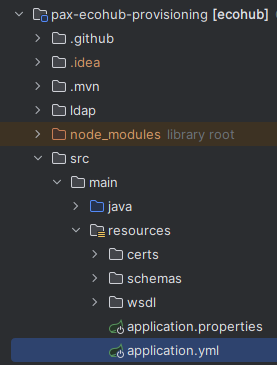
\includegraphics[width=0.4\textwidth]{images/applicationYAMLOrt.png}
    \caption{Pfad zur \texttt{application.yml}-Datei}
    \label{fig:patchYmlFile}
\end{figure}


\subsection{Entfernen des Nutzers aus bestehenden Gruppen}

Bevor ein Nutzer auf Basis seiner neuen Rollen den zugehörigen Gruppen zugeordnet werden kann, muss er aus allen Gruppen entfernt werden, in denen er möglicherweise noch eingetragen ist. Dies stellt sicher, dass keine veralteten oder mehrfachen Gruppenzugehörigkeiten bestehen.

\subsubsection*{Zweck der Methode}
Die Methode \texttt{removeUserFromAllGroup} entfernt einen Nutzer anhand seines sogenannten \textit{Distinguished Name (DN)} aus allen Gruppen, die über das Rollenkonfigurations-Mapping bekannt sind. Die Methode befindet sich in der Datei \texttt{PersonRepositoryImpl.java}.

\subsubsection*{Aufbau der Methode}
Die Methode ist in mehrere sinnvolle Teilschritte gegliedert, die im Folgenden einzeln erklärt werden.

\paragraph{1. Zusammensetzen des vollständigen Benutzer-DN}
Damit der Nutzer in den LDAP-Gruppen eindeutig identifiziert werden kann, muss sein DN vollständig angegeben werden. Dazu wird an den mitgegebenen DN-Teil der Domänenteil \texttt{dc=paxportal,dc=person} angehängt:

\begin{lstlisting}[language=Java, caption={Konstruktion des vollständigen Benutzer-DN}]
userDn = userDn + "dc=paxportal,dc=person";
\end{lstlisting}

\paragraph{2. Ermittlung aller bekannten Gruppen}
Statt alle Gruppen manuell aufzulisten, wird hier dynamisch aus der bestehenden Rollenkonfiguration (`roleMappings`) ermittelt, welche Gruppen existieren. So ist die Methode flexibel erweiterbar, ohne Änderungen im Code:

\begin{lstlisting}[language=Java, caption={Dynamisches Sammeln aller Zielgruppen}]
    Set<String> allGroups = new HashSet<>();
    for (List<String> groups : getRoleMappings().values()) {
        allGroups.addAll(groups);
    }
\end{lstlisting}

\paragraph{3. Entfernen des Nutzers aus jeder Gruppe}
Für jede gefundene Gruppe wird versucht, den Nutzer aus dem Gruppenobjekt zu entfernen. Dies geschieht über eine LDAP-Änderungsoperation, bei der der `member`-Eintrag des Nutzers gelöscht wird. Falls der Nutzer nicht in der Gruppe enthalten ist oder ein Fehler auftritt, wird dies protokolliert, aber die Ausführung geht weiter:

\begin{lstlisting}[language=Java, caption={LDAP-Entfernungsvorgang für Gruppenmitgliedschaft}]
    for (String groupDn : allGroups) {
        try {
            ModificationItem[] mods = new ModificationItem[] {
                new ModificationItem(DirContext.REMOVE_ATTRIBUTE, new BasicAttribute("member", userDn))
            };

            ldapTemplate.modifyAttributes(groupDn, mods);
            log.info("Remove user from group [userDn={}, groupDn={}]", userDn, groupDn);
        } catch (Exception e) {
            log.debug("User not in group or other error. [userDn={}, groupDn={}, exception={}]",
                    userDn, groupDn, e.getMessage());
        }
    }
\end{lstlisting}

\paragraph{4. Rückmeldung über Erfolg oder Fehler}
Zum Schluss gibt die Methode einen \texttt{boolean}-Wert zurück. Dieser signalisiert, ob der gesamte Entfernungsvorgang erfolgreich war oder ob ein Fehler auftrat:

\begin{lstlisting}[language=Java, caption={Fehlerbehandlung und Rückgabewert}]
    log.info("Remove user from group [userDn={}]", userDn);
    return true;
    } catch (Exception e) {
        log.error("Failed to remove user from groups. [userDn={}, exception={}]", userDn, e.getMessage());
        return false;
    }
\end{lstlisting}

\subsubsection*{Fazit}
Die Methode \texttt{removeUserFromAllGroup} sorgt für einen sauberen Ausgangszustand, indem sie alle bestehenden Gruppenzugehörigkeiten eines Nutzers entfernt. Damit wird sichergestellt, dass nachfolgende Zuweisungen (siehe nächste Subsection) konsistent und fehlerfrei erfolgen können. Durch die dynamische Ermittlung der Gruppen ist die Methode flexibel und wartungsarm.

\clearpage
\subsubsection{Die komplette removeUserFromAllGroup Methode}
Hier die komplette \texttt{removeUserFromAllGroup} Methode:
\begin{lstlisting}[language=Java, caption={Die komplette removeUserFromAllGroup Methode}, label={lst:removeUserFromAllGroup}]
    private boolean removeUserFromAllGroup(String userDn) {
        userDn = userDn + "dc=paxportal,dc=person";
        try {
            Set<String> allGroups = new HashSet<>();
            for (List<String> groups : getRoleMappings().values()) {
                allGroups.addAll(groups);
            }

            for (String groupDn : allGroups) {
                try {
                    ModificationItem[] mods = new ModificationItem[] {
                            new ModificationItem(DirContext.REMOVE_ATTRIBUTE, new BasicAttribute("member", userDn))
                    };

                    ldapTemplate.modifyAttributes(groupDn, mods);
                    log.info("Remove user from group [userDn={}, groupDn={}]", userDn, groupDn);
                } catch (Exception e) {
                    log.debug("User not in group or other error. [userDn={}, groupDn={}, exception={}]",
                            userDn, groupDn, e.getMessage());
                }
            }

            log.info("Remove user from group [userDn={}]", userDn);
            return true;
        } catch (Exception e) {
            log.error("Failed to remove user from groups. [userDn={}, exception={}]", userDn, e.getMessage());
            return false;
        }
    }
\end{lstlisting}

\subsection{Hinzufügen des Nutzers zu den neuen Gruppen}

Nachdem der Nutzer aus allen bestehenden LDAP-Gruppen entfernt wurde (siehe Abschnitt~\ref{lst:removeUserFromAllGroups}), wird er in einem zweiten Schritt wieder den richtigen Gruppen zugewiesen. Dies geschieht auf Basis der Rollen, die im sogenannten \texttt{CompleteUserType}-Objekt übermittelt werden. Die zentrale Methode für diese Aufgabe heisst \texttt{updateUserGroup} und befindet sich in der Datei \texttt{PersonRepositoryImpl.java}.

\subsubsection*{Zweck der Methode}
Die Methode analysiert die Rollen des Nutzers (\texttt{igRoles}), vergleicht sie mit der Konfiguration aus der \texttt{application.yml}, und fügt den Nutzer dann den passenden Gruppen im LDAP hinzu.

\subsubsection*{Aufbau der Methode}
Im Folgenden werden die wichtigsten Bestandteile der Methode schrittweise erklärt und jeweils mit einem Codeausschnitt ergänzt.

\paragraph{1. Vorbereitung und Abbruch bei fehlenden Rollen}
Zu Beginn wird überprüft, ob der Nutzer überhaupt Rollen besitzt. Falls keine vorhanden sind, wird der Vorgang übersprungen:

\begin{lstlisting}[language=Java, caption={Abbruch bei fehlenden Rolleninformationen}]
    if (payload == null || payload.getIgRoles() == null || payload.getIgRoles().isEmpty()) {
        log.info("No igRoles provided, skipping group updates");
        return;
    }
\end{lstlisting}

\paragraph{2. Ermittlung der Zielgruppen basierend auf Rollenpräfixen}
Es wird eine Liste von Zielgruppen aufgebaut. Dafür werden alle Rollen mit den definierten Präfixen (z.\,B. \texttt{EL\_}, \texttt{KL\_}) verglichen. Jede passende Rolle führt zur Zuordnung der zugehörigen Gruppen:

\begin{lstlisting}[language=Java, caption={Zuordnung der Rollen zu Gruppen}]
    Map<String, Boolean> targetGroups = new HashMap<>();
    List<String> igRoles = payload.getIgRoles();

    for (String igRole : igRoles) {
        for (Map.Entry<String, List<String>> entry : getRoleMappings().entrySet()) {
            String prefix = entry.getKey();
            List<String> groups = entry.getValue();

            if (igRole.startsWith(prefix)) {
                for (String groupDn : groups) {
                    targetGroups.put(groupDn, true);
                }
            }
        }
    }
\end{lstlisting}

\paragraph{3. Nutzer wird zu jeder relevanten Gruppe hinzugefügt}
Für jede ermittelte Gruppe wird eine LDAP-Operation ausgeführt, die den Nutzer der Gruppe hinzufügt. Diese Operation wird mit einer sogenannten \texttt{ModificationItem}-Anweisung durchgeführt:

\begin{lstlisting}[language=Java, caption={Hinzufügen des Nutzers zu den LDAP-Gruppen}]
    for (String groupDn : targetGroups.keySet()) {
        try {
            ModificationItem[] mods = new ModificationItem[] {
                new ModificationItem(DirContext.ADD_ATTRIBUTE, new BasicAttribute("member", userDn))
            };

            ldapTemplate.modifyAttributes(groupDn, mods);
            log.info("Added user to group. [userDn={}, groupDn={}]", userDn, groupDn);
        } catch (Exception e) {
            log.error("Failed to add user to group. [userDn={}, groupDn={}, exception={}, cause={}]",
                    userDn, groupDn, e.getMessage(), e.getCause() != null ? e.getCause().getMessage() : "none");
        }
    }
\end{lstlisting}

\paragraph{4. Fehlerbehandlung}
Die gesamte Methode ist zusätzlich in einen \texttt{try-catch}-Block gehüllt, um bei allgemeinen Fehlern während der Gruppenverarbeitung ein Logging vorzunehmen:

\begin{lstlisting}[language=Java, caption={Allgemeine Fehlerbehandlung am Ende der Methode}]
    } catch (Exception e) {
        log.error("Failed to update user groups. [userDn={}, exception={}]", userDn, e.getMessage());
    }
\end{lstlisting}

\subsubsection*{Fazit}
Die Methode \texttt{updateUserGroup} ist zentral für die automatische rollenbasierte Gruppensteuerung im LDAP. Sie stellt sicher, dass ein Nutzer nach dem Update nur noch in den Gruppen enthalten ist, die seiner aktuellen Rollenstruktur entsprechen. Dabei wird auf Konfigurierbarkeit über die YAML-Datei gesetzt, wodurch die Lösung flexibel erweitert werden kann.

\clearpage
\subsubsection{Die komplette updateUserGroup Methode}
Hier die komplette \texttt{updateUserGroup} Methode:
\begin{lstlisting}[language=Java, caption={Die komplette updateUserGroup Methode}, label={lst:updateUserGroup}]
    private void updateUserGroup(String userDn, final CompleteUserType payload) {
        userDn = userDn + ",dc=paxportal,dc=ch";
        if (payload == null || payload.getIgRoles() == null || payload.getIgRoles().isEmpty()) {
            log.info("No igRoles provided, skipping group updates");
            return;
        }

        try {
            Map<String, Boolean> targetGroups = new HashMap<>();
            List<String> igRoles = payload.getIgRoles();

            for (String igRole : igRoles) {
                for (Map.Entry<String, List<String>> entry : getRoleMappings().entrySet()){
                    String prefix = entry.getKey();
                    List<String> groups = entry.getValue();

                    if (igRole.startsWith(prefix)) {
                        for (String groupDn : groups) {
                            targetGroups.put(groupDn, true);
                        }
                    }
                }
            }

            for (String groupDn : targetGroups.keySet()) {
                try {
                    ModificationItem[] mods = new ModificationItem[] {
                            new ModificationItem(DirContext.ADD_ATTRIBUTE, new BasicAttribute("member", userDn))
                    };

                    log.debug("Attempting to add user to group. [userDn={}, groupDn={}]", userDn, groupDn);
                    ldapTemplate.modifyAttributes(groupDn, mods);
                    log.info("Added user to group. [userDn={}, groupDn={}]", userDn, groupDn);
                } catch (Exception e) {
                    log.error("Failed to add user to group. [userDn={}, groupDn={}, exception={}, cause={}]",
                            userDn, groupDn, e.getMessage(), e.getCause() != null ? e.getCause().getMessage() : "none");
                }
            }

            log.info("Remove user from group [userDn={}]", userDn);
        } catch (Exception e) {
            log.error("Failed to update user groups. [userDn={}, exception={}]", userDn, e.getMessage());
        }
    }
\end{lstlisting}

\subsection{Einbindung der Mapping-Funktionen in \texttt{updateUser}}

Die zuvor beschriebenen Methoden \texttt{removeUserFromAllGroup} und \texttt{updateUserGroup} werden innerhalb der zentralen \texttt{updateUser}-Funktion aufgerufen. Diese Funktion wird verwendet, wenn bestehende Benutzer im LDAP-Verzeichnis aktualisiert werden sollen.

Dabei erfolgt die Gruppenverwaltung in drei aufeinanderfolgenden Schritten:

\begin{enumerate}
  \item Änderung der Basisattribute des Benutzers (z.\,B. IDP-Nummer)
  \item Entfernen des Benutzers aus allen Gruppen
  \item Neue Gruppenzuweisung basierend auf den aktuellen Rollen
\end{enumerate}

\noindent Die folgende Methode zeigt die vollständige Integration:

\begin{lstlisting}[language=Java, caption={updateUser-Methode mit eingebauten Mapping-Funktionen}, label={lst:updateUser}]
    @Override
    public boolean updatePerson(final Person person, final CompleteUserType payload) {
        final String idpUserId = payload.getIdpUserId();
        boolean updated = false;
        log.info("Update person in LDAP started. [idpUserId={}]", idpUserId);

        try {
            ldapTemplate.modifyAttributes(person.getDn(), buildModification(idpUserId));

            boolean removalSuccess = removeUserFromAllGroup(person.getDn().toString());
            if (!removalSuccess) {
                log.error("Failed to remove user from groups. [idpUserId={}]", idpUserId);
                return false;
            }

            updateUserGroup(person.getDn().toString(), payload);

            log.info("Update person in LDAP succeeded. [idpUserId={}]", idpUserId);
            updated = true;

        } catch (final Exception e) {
            log.info("Update person in LDAP failed. [idpUserId={}, exception={}]", idpUserId, e.getMessage());
        }

        log.info("Update person in LDAP finished. [idpUserId={}]", idpUserId);
        return updated;
    }
\end{lstlisting}

\subsubsection*{Erläuterung der Abläufe}

\begin{itemize}
    \item \texttt{modifyAttributes(...)}: Aktualisiert z.\,B. die IDP-Nummer des Nutzers im LDAP.
    \item \texttt{removeUserFromAllGroup(...)}: Entfernt den Nutzer aus allen Gruppen, basierend auf dem aktuellen Rollenkontext.
    \item \texttt{updateUserGroup(...)}: Fügt den Nutzer anhand der Rollen (\texttt{igRoles}) den in der YAML-Konfiguration definierten Gruppen hinzu.
\end{itemize}

\noindent Diese Einbettung stellt sicher, dass jeder Benutzer nach einem Update nur genau in den Gruppen enthalten ist, die seiner aktuellen Rolle entsprechen.
